\chapter{Travaux précédents (Zoé Marcelet)}
\label{ch:Ch1}

%%%%%%%%%%%%%%%%%%%%%%%%%%%%%%%%%%%% SECTION 1
\section{Modèle Lagragien} 
\label{sec:Ch1.1}

D'après le document \textit{"Dynamics and Control of Single-Line Kites"} de Gonzalo Sanchez-Arriaga (2006),  les formules suivantes permettent d'obtenir l'élévation $\Gamma$ et l'angle d'incidence du vent $\theta$, en fonction du vent et des coefficients aérodynamiques du kite : \\

\begin{figure}[H]
    \centering
    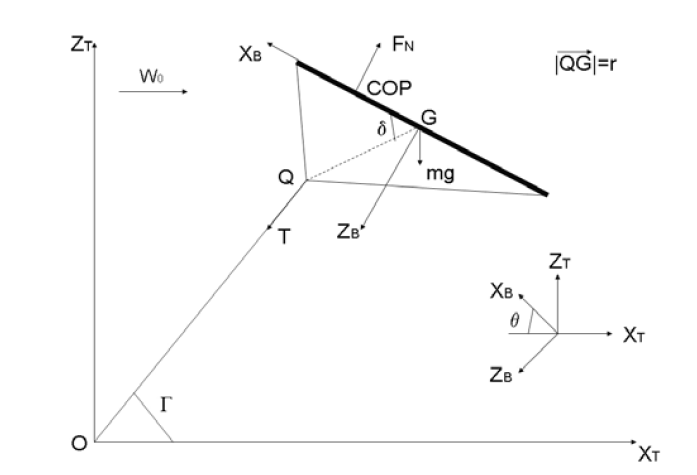
\includegraphics[width=0.5\textwidth]{Pics/01 - Travaux précédents/Picture Sanchez.png}  
    \caption{Schéma du kite au Zénith.}
    \label{fig:sanchez}
\end{figure}

La première équation donne l’angle d’incidence $\theta$ : 
\begin{center}
    \begin{equation}
        cos(\delta - \theta) + \beta (\sigma-cos(\delta))C_N(\theta) = 0
        \label{eq:theta}
    \end{equation}
\end{center}
La deuxieme équation donne l’angle d’élévation $\Gamma$ :
\begin{center}
    \begin{equation}
        \Gamma = tan^{-1}(\frac{\beta C_N (\theta) cos(\theta)-1}{\beta C_N (\theta)sin(\theta)})
        \label{eq:gamma}
    \end{equation}
\end{center}
Avec $\beta = \frac{\rho A W_0^2}{2mg}$ et $\sigma = \frac{X_{cp}}{r}$ \\

Ces équations ont été codées (disponible sur Nextcloud : 06-RESSOURCE/AC-Admin Commun/4-Rapports Stagiaires/Stage Zoé Marcelet/Rapport\_zozo/06\_Topic\_modèle\_aéro\_zenith). \\
\textbf{Elles restent cependant peut concluantes car requièrent les coéfficients aérodynamiques du kite. }